\chapter{Attention Mechanisms and Transformers}
\label{chap:attention_transformers}

\begin{tldr}
Attention mechanisms enable neural networks to dynamically focus on relevant parts of the input. This chapter covers the mathematical foundations of attention (additive, multiplicative, scaled dot-product), self-attention and multi-head attention, the complete Transformer architecture, positional encodings (sinusoidal, learned, RoPE, ALiBi), efficient attention variants (sparse, linear, Flash Attention), and modern design choices (pre-norm, GQA, SwiGLU). Understanding attention deeply---including computational complexity and memory requirements---is essential for staff-level ML interviews.
\end{tldr}

\section{Attention as a Computational Primitive}
\label{sec:attention_primitive}

\subsection{The Core Intuition}

Attention can be understood as a \textbf{soft dictionary lookup}:

\begin{itemize}
    \item \textbf{Query} ($\vq$): What you're looking for
    \item \textbf{Keys} ($\vk$): What each item ``is'' (index)
    \item \textbf{Values} ($\vv$): What information to retrieve
\end{itemize}

\begin{equation}
\text{output} = \sum_i \underbrace{\text{similarity}(\vq, \vk_i)}_{\text{attention weight}} \cdot \vv_i
\end{equation}

Unlike hard dictionary lookup (exact match), attention computes a weighted combination based on similarity.

\subsection{Mathematical Formulation}

\begin{definition}[General Attention]
Given query $\vq \in \R^{d_q}$, keys $\mK \in \R^{n \times d_k}$, and values $\mV \in \R^{n \times d_v}$:
\begin{equation}
\text{Attention}(\vq, \mK, \mV) = \sum_{i=1}^{n} \alpha_i \vv_i = \bm{\alpha}^T \mV
\end{equation}
where attention weights $\bm{\alpha} = \softmax(\bm{e})$ and $\bm{e} = [e_1, \ldots, e_n]$ are alignment scores.
\end{definition}

The choice of alignment function $e_i = f(\vq, \vk_i)$ defines different attention mechanisms.

%==============================================================================
\section{Types of Attention Mechanisms}
\label{sec:attention_types}
%==============================================================================

\subsection{Additive (Bahdanau) Attention}

\begin{mathresult}{Additive Attention}
\begin{equation}
e_i = \vv_a^T \tanh(\mW_q \vq + \mW_k \vk_i + \vb)
\end{equation}
where $\mW_q \in \R^{d_a \times d_q}$, $\mW_k \in \R^{d_a \times d_k}$, and $\vv_a \in \R^{d_a}$.
\end{mathresult}

\textbf{Properties}:
\begin{itemize}
    \item Parameters: $d_a(d_q + d_k + 1)$
    \item Allows different query and key dimensions
    \item More expressive (nonlinear combination)
    \item Slower due to the MLP
\end{itemize}

\textbf{Historical context}: Introduced in the seminal neural machine translation paper (Bahdanau et al., 2014).

\subsection{Multiplicative (Luong) Attention}

\begin{mathresult}{Multiplicative Attention Variants}
\begin{align}
\text{Dot:} \quad e_i &= \vq^T \vk_i \\
\text{General:} \quad e_i &= \vq^T \mW \vk_i \\
\text{Bilinear:} \quad e_i &= \vq^T \mW \vk_i + \vw^T[\vq; \vk_i] + b
\end{align}
\end{mathresult}

\textbf{Properties}:
\begin{itemize}
    \item Simpler, faster (no nonlinearity)
    \item Dot product requires $d_q = d_k$
    \item General form adds expressivity with $\mW$
\end{itemize}

\subsection{Scaled Dot-Product Attention}

\begin{mathresult}{Scaled Dot-Product Attention}
\begin{equation}
\text{Attention}(\mQ, \mK, \mV) = \softmax\left(\frac{\mQ\mK^T}{\sqrt{d_k}}\right)\mV
\end{equation}
\end{mathresult}

This is the attention mechanism used in Transformers.

\subsubsection{Why Scale by $\sqrt{d_k}$?}

Without scaling, dot products grow with dimension $d$ (their variance equals $d$). This pushes softmax into saturation where gradients vanish. Dividing by $\sqrt{d_k}$ restores unit variance and keeps gradients healthy.

\begin{figure}[H]
\centering
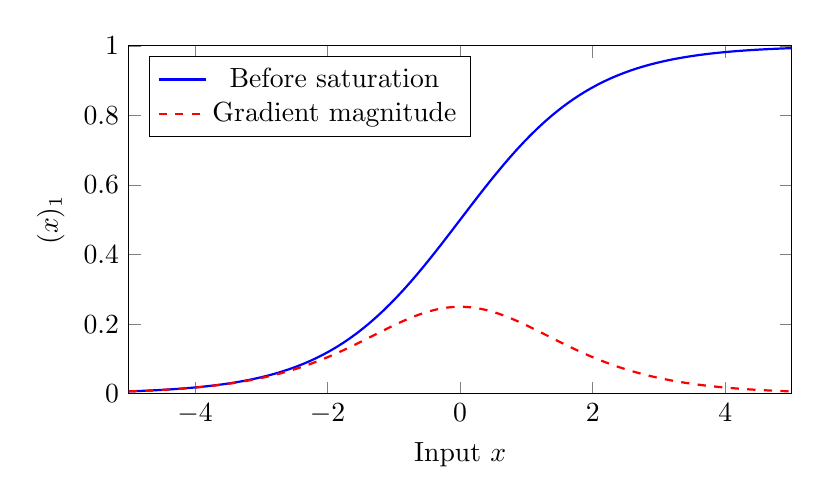
\begin{tikzpicture}
    \begin{axis}[
        xlabel={Input $x$},
        ylabel={$\softmax(x)_1$},
        xmin=-5, xmax=5,
        ymin=0, ymax=1,
        legend pos=north west,
        width=10cm,
        height=6cm
    ]
    % For 2 classes, softmax(x) vs softmax(-x)
    \addplot[domain=-5:5, samples=100, thick, blue] {exp(x)/(exp(x)+exp(0))};
    \addlegendentry{Before saturation}

    % Gradient visualization
    \addplot[domain=-5:5, samples=100, thick, red, dashed] {exp(x)/(exp(x)+exp(0)) * (1 - exp(x)/(exp(x)+exp(0)))};
    \addlegendentry{Gradient magnitude}
    \end{axis}
\end{tikzpicture}
\caption{Softmax output and gradient. Large inputs cause saturation where gradients vanish.}
\label{fig:softmax_saturation}
\end{figure}

%==============================================================================
\section{Self-Attention}
\label{sec:self_attention}
%==============================================================================

\subsection{Definition}

In self-attention, queries, keys, and values all come from the same sequence:

\begin{mathresult}{Self-Attention}
Given input sequence $\mX \in \R^{n \times d}$:
\begin{align}
\mQ &= \mX \mW^Q, \quad \mK = \mX \mW^K, \quad \mV = \mX \mW^V \\
\text{SelfAttention}(\mX) &= \softmax\left(\frac{\mQ\mK^T}{\sqrt{d_k}}\right)\mV
\end{align}
where $\mW^Q, \mW^K \in \R^{d \times d_k}$ and $\mW^V \in \R^{d \times d_v}$.
\end{mathresult}

\subsection{What Self-Attention Computes}

For each position $i$:
\begin{equation}
\vy_i = \sum_{j=1}^n \alpha_{ij} \vv_j
\end{equation}
where $\alpha_{ij} = \softmax_j\left(\frac{\vq_i^T \vk_j}{\sqrt{d_k}}\right)$.

\textbf{Interpretation}: Position $i$'s output is a weighted combination of all positions' values, weighted by query-key similarity.

\subsection{Computational Complexity}

\textbf{Self-Attention Complexity.}
For sequence length $n$ and dimension $d$:
\begin{itemize}
    \item \textbf{Time}: $O(n^2 d)$ for attention scores + $O(n^2 d)$ for weighted sum = $O(n^2 d)$
    \item \textbf{Memory}: $O(n^2)$ for attention matrix + $O(nd)$ for embeddings
\end{itemize}

The $O(n^2)$ complexity is the fundamental limitation for long sequences.

\subsection{Properties of Self-Attention}

\begin{enumerate}
    \item \textbf{Permutation equivariant}: $\text{SelfAttn}(\pi(\mX)) = \pi(\text{SelfAttn}(\mX))$
    \begin{itemize}
        \item The operation itself doesn't know position
        \item Position must be injected via positional encodings
    \end{itemize}

    \item \textbf{Global receptive field}: Every position can attend to every other position from layer 1
    \begin{itemize}
        \item Unlike CNNs (local) or RNNs (sequential)
        \item Enables modeling long-range dependencies
    \end{itemize}

    \item \textbf{Dynamic}: Attention pattern depends on input content
    \begin{itemize}
        \item Unlike convolution with fixed kernel
        \item Can learn different patterns for different inputs
    \end{itemize}
\end{enumerate}

%==============================================================================
\section{Multi-Head Attention}
\label{sec:multi_head}
%==============================================================================

\subsection{Motivation}

Single attention head learns one type of relationship. Multiple heads learn diverse patterns:
\begin{itemize}
    \item Some heads focus on local context
    \item Some heads capture long-range dependencies
    \item Different heads for different syntactic/semantic roles
\end{itemize}

\subsection{Mathematical Formulation}

\begin{mathresult}{Multi-Head Attention}
\begin{align}
\text{MultiHead}(\mQ, \mK, \mV) &= \text{Concat}(\text{head}_1, \ldots, \text{head}_h)\mW^O \\
\text{head}_i &= \text{Attention}(\mQ\mW_i^Q, \mK\mW_i^K, \mV\mW_i^V)
\end{align}
where $\mW_i^Q, \mW_i^K \in \R^{d \times d_k}$, $\mW_i^V \in \R^{d \times d_v}$, $\mW^O \in \R^{hd_v \times d}$, and typically $d_k = d_v = d/h$.
\end{mathresult}

\subsection{Implementation Detail}

\textbf{Efficient computation}: Instead of $h$ separate attention operations:
\begin{enumerate}
    \item Project $\mQ, \mK, \mV$ to shape $(n, h, d_k)$
    \item Transpose to $(h, n, d_k)$ for batched matrix multiplication
    \item Compute all heads in parallel
    \item Concatenate and project
\end{enumerate}

\subsection{Parameter Count}

For model dimension $d$ with $h$ heads:
\begin{align}
\mW^Q, \mW^K, \mW^V &: 3 \times d \times d = 3d^2 \\
\mW^O &: d \times d = d^2 \\
\text{Total} &: 4d^2
\end{align}

\subsection{What Different Heads Learn}

Empirical observations:
\begin{itemize}
    \item \textbf{Positional heads}: Attend to fixed relative positions
    \item \textbf{Syntactic heads}: Subject-verb, modifier-noun relationships
    \item \textbf{Rare word heads}: Attend to infrequent tokens
    \item \textbf{Delimiter heads}: Attend to [SEP], periods
    \item \textbf{Previous/next token heads}: Local context
\end{itemize}

%==============================================================================
\section{The Transformer Architecture}
\label{sec:transformer_arch}
%==============================================================================

\subsection{Overview}

\begin{figure}[H]
\centering
\begin{tikzpicture}[
    node distance=0.7cm,
    box/.style={rectangle, draw, minimum width=3cm, minimum height=0.7cm, rounded corners},
    block/.style={box, fill=lightblue},
    norm/.style={box, fill=lightyellow, minimum width=2.5cm},
    ffn/.style={box, fill=lightgreen},
    input/.style={box, fill=lightgray},
    attention/.style={box, fill=orange!30}
]
    % Input
    \node[input] (input) {Input Embeddings + Position};

    % Encoder block
    \node[attention, above=0.5cm of input] (attn1) {Multi-Head Self-Attention};
    \node[norm, above=0.3cm of attn1] (norm1) {Add \& LayerNorm};
    \node[ffn, above=0.3cm of norm1] (ffn1) {Feed-Forward Network};
    \node[norm, above=0.3cm of ffn1] (norm2) {Add \& LayerNorm};

    % Block indicator
    \draw[thick, decorate, decoration={brace, amplitude=10pt, raise=5pt}]
        ($(attn1.south west)+(-0.5,0)$) -- ($(norm2.north west)+(-0.5,0)$)
        node[midway, left=15pt, font=\small] {$\times N$};

    % Output
    \node[above=0.5cm of norm2] (output) {To next layer / Output};

    % Residual connections
    \draw[->] (input) -- (attn1);
    \draw[->] (attn1) -- (norm1);
    \draw[->] (norm1) -- (ffn1);
    \draw[->] (ffn1) -- (norm2);
    \draw[->] (norm2) -- (output);

    % Residual arrows
    \draw[->, dashed, gray] (input.east) -- ++(0.8,0) |- (norm1.east);
    \draw[->, dashed, gray] (norm1.east) -- ++(0.5,0) |- (norm2.east);

\end{tikzpicture}
\caption{Single Transformer encoder block (post-norm variant).}
\label{fig:transformer_block}
\end{figure}

\subsection{Encoder Block}

Each encoder block consists of:

\begin{enumerate}
    \item \textbf{Multi-Head Self-Attention}
    \begin{equation}
    \tilde{\mH} = \text{MultiHeadAttention}(\mH, \mH, \mH)
    \end{equation}

    \item \textbf{Residual Connection + Layer Normalization}
    \begin{equation}
    \mH' = \text{LayerNorm}(\mH + \tilde{\mH})
    \end{equation}

    \item \textbf{Position-wise Feed-Forward Network}
    \begin{equation}
    \text{FFN}(\vx) = \mW_2 \cdot \sigma(\mW_1 \vx + \vb_1) + \vb_2
    \end{equation}
    Typically with expansion factor 4: $\mW_1 \in \R^{d \times 4d}$, $\mW_2 \in \R^{4d \times d}$.

    \item \textbf{Another Residual + LayerNorm}
    \begin{equation}
    \mH'' = \text{LayerNorm}(\mH' + \text{FFN}(\mH'))
    \end{equation}
\end{enumerate}

\subsection{Decoder Block}

Decoder adds:
\begin{enumerate}
    \item \textbf{Masked Self-Attention}: Prevents attending to future positions
    \item \textbf{Cross-Attention}: Attends to encoder outputs
\end{enumerate}

\begin{mathresult}{Causal Mask}
\begin{equation}
M_{ij} = \begin{cases}
0 & \text{if } j \leq i \\
-\infty & \text{if } j > i
\end{cases}
\end{equation}
Applied as: $\softmax\left(\frac{\mQ\mK^T}{\sqrt{d_k}} + \mathbf{M}\right)$
\end{mathresult}

\subsection{Pre-Norm vs Post-Norm}

\textbf{Post-Norm (Original Transformer)}:
\begin{equation}
\mH' = \text{LayerNorm}(\mH + \text{SubLayer}(\mH))
\end{equation}

\textbf{Pre-Norm (Modern Standard)}:
\begin{equation}
\mH' = \mH + \text{SubLayer}(\text{LayerNorm}(\mH))
\end{equation}

\begin{table}[H]
\centering
\caption{Pre-Norm vs Post-Norm comparison}
\begin{tabularx}{\textwidth}{lXX}
\toprule
\textbf{Aspect} & \textbf{Post-Norm} & \textbf{Pre-Norm} \\
\midrule
Gradient flow & Through LayerNorm & Direct residual path \\
Training stability & Needs warmup & More stable \\
Final performance & Slightly better (when stable) & Very close \\
Modern usage & Rare & Standard (GPT, LLaMA, etc.) \\
\bottomrule
\end{tabularx}
\end{table}

\begin{keyinsight}{Why Pre-Norm Stabilizes Training}
Pre-norm is more stable because the residual path doesn't pass through normalization:
\begin{equation}
\frac{\partial \loss}{\partial \mH} = \frac{\partial \loss}{\partial \mH'} \cdot \left(\mI + \frac{\partial \text{SubLayer}}{\partial \mH}\right)
\end{equation}
The identity term $\mI$ ensures gradient always flows, preventing vanishing gradients.
\end{keyinsight}

%==============================================================================
\section{Positional Encodings}
\label{sec:positional}
%==============================================================================

\subsection{Why Position Information is Needed}

Self-attention is \textbf{permutation equivariant}:
\begin{equation}
\text{SelfAttn}(\pi(\mX)) = \pi(\text{SelfAttn}(\mX))
\end{equation}

Without positional information, ``The cat sat on the mat'' and ``mat the on sat cat The'' produce the same output!

\subsection{Sinusoidal Positional Encoding}

\begin{mathresult}{Sinusoidal Encoding (Original Transformer)}
\begin{align}
PE_{(pos, 2i)} &= \sin\left(\frac{pos}{10000^{2i/d}}\right) \\
PE_{(pos, 2i+1)} &= \cos\left(\frac{pos}{10000^{2i/d}}\right)
\end{align}
\end{mathresult}

\textbf{Properties}:
\begin{itemize}
    \item Deterministic, no learned parameters
    \item Each dimension has different frequency
    \item Can extrapolate to longer sequences than seen in training
\end{itemize}

\textbf{Why it enables relative position}:
For any fixed offset $k$:
\begin{equation}
PE_{pos+k} = f_k(PE_{pos})
\end{equation}
where $f_k$ is a linear transformation (rotation matrix). This allows the model to learn to attend to relative positions.

\subsection{Learned Positional Embeddings}

\begin{equation}
\mE_{pos} \in \R^{L_{max} \times d}
\end{equation}
Learn embedding for each position up to maximum length $L_{max}$.

\textbf{Used in}: BERT, GPT-2

\textbf{Limitation}: Cannot extrapolate beyond $L_{max}$.

\subsection{Relative Positional Encodings}

\subsubsection{Shaw et al. Relative Attention}

Add relative position embeddings to keys:
\begin{equation}
e_{ij} = \frac{(\vx_i \mW^Q)(\vx_j \mW^K + \va_{j-i}^K)^T}{\sqrt{d_k}}
\end{equation}

Optionally also to values:
\begin{equation}
\vz_i = \sum_j \alpha_{ij}(\vx_j \mW^V + \va_{j-i}^V)
\end{equation}

\textbf{Used in}: Transformer-XL, T5

\subsection{Rotary Position Embedding (RoPE)}

\begin{mathresult}{RoPE}
Encode position by rotating query and key vectors:
\begin{equation}
f(\vx, m) = \mR_m \vx
\end{equation}
where $\mR_m$ is a rotation matrix dependent on position $m$.
\end{mathresult}

For 2D subspaces:
\begin{equation}
\mR_m = \begin{pmatrix}
\cos(m\theta_1) & -\sin(m\theta_1) & & \\
\sin(m\theta_1) & \cos(m\theta_1) & & \\
& & \ddots & \\
& & & \cos(m\theta_{d/2}) & -\sin(m\theta_{d/2}) \\
& & & \sin(m\theta_{d/2}) & \cos(m\theta_{d/2})
\end{pmatrix}
\end{equation}

\textbf{Key property}: Relative position naturally encoded:
\begin{equation}
(\mR_m \vq)^T (\mR_n \vk) = \vq^T \mR_m^T \mR_n \vk = \vq^T \mR_{n-m} \vk
\end{equation}

\textbf{Used in}: LLaMA, Mistral, most modern open LLMs

\textbf{Advantages}:
\begin{itemize}
    \item No explicit position embeddings
    \item Naturally encodes relative positions
    \item Good extrapolation
    \item Efficient implementation
\end{itemize}

\begin{warningbox}
Positional encoding extrapolation is not free. A model trained with 4K context won't magically work at 32K just because it uses RoPE or ALiBi. You still need position interpolation, continued pre-training, or progressive extension to reliably handle longer contexts.
\end{warningbox}

\subsection{ALiBi (Attention with Linear Biases)}

\begin{mathresult}{ALiBi}
Add linear bias based on distance:
\begin{equation}
\text{softmax}\left(\frac{\vq_i^T \vk_j}{\sqrt{d_k}} - m \cdot |i - j|\right)
\end{equation}
where $m$ is a head-specific slope.
\end{mathresult}

\textbf{Properties}:
\begin{itemize}
    \item No position embeddings at all
    \item Linear penalty for distance
    \item Excellent length extrapolation
    \item Different heads have different ``attention spans''
\end{itemize}

\textbf{Used in}: BLOOM, MPT

\subsection{Positional Encoding Comparison}

\begin{table}[H]
\centering
\caption{Positional encoding comparison}
\begin{tabularx}{\textwidth}{lXXXX}
\toprule
\textbf{Encoding} & \textbf{Parameters} & \textbf{Extrapolation} & \textbf{Relative} & \textbf{Used In} \\
\midrule
Sinusoidal & None & Good & Implicit & Original Transformer \\
Learned & $L \times d$ & Poor & No & BERT, GPT-2 \\
Relative (Shaw) & $O(Ld)$ & Moderate & Explicit & T5, XL \\
RoPE & None & Good & Implicit & LLaMA, Mistral \\
ALiBi & $h$ scalars & Excellent & Implicit & BLOOM, MPT \\
\bottomrule
\end{tabularx}
\end{table}

%==============================================================================
\section{Efficient Attention Variants}
\label{sec:efficient_attention}
%==============================================================================

\subsection{The Efficiency Challenge}

Standard attention: $O(n^2)$ time and memory

\begin{table}[H]
\centering
\caption{Memory requirements for attention at different scales}
\begin{tabular}{lrrr}
\toprule
\textbf{Sequence Length} & \textbf{Attention Matrix} & \textbf{At FP16} & \textbf{At FP32} \\
\midrule
512 & 262K elements & 0.5 MB & 1 MB \\
2,048 & 4.2M elements & 8 MB & 16 MB \\
8,192 & 67M elements & 128 MB & 256 MB \\
32,768 & 1.07B elements & 2 GB & 4 GB \\
131,072 & 17B elements & 32 GB & 64 GB \\
\bottomrule
\end{tabular}
\end{table}

\subsection{Sparse Attention Patterns}

\subsubsection{Local/Sliding Window Attention}

Each position attends only to a window of $w$ neighbors:
\begin{equation}
\alpha_{ij} = 0 \text{ if } |i - j| > w/2
\end{equation}

\textbf{Complexity}: $O(nw)$

\textbf{Used in}: Longformer (with global tokens), Mistral

\subsubsection{Dilated Attention}

Attend to positions at fixed intervals, similar to dilated convolutions.

\subsubsection{Global + Local (Longformer/BigBird)}

\begin{itemize}
    \item Most positions: Local attention (window)
    \item Special tokens (CLS, etc.): Global attention to all positions
\end{itemize}

\begin{figure}[H]
\centering
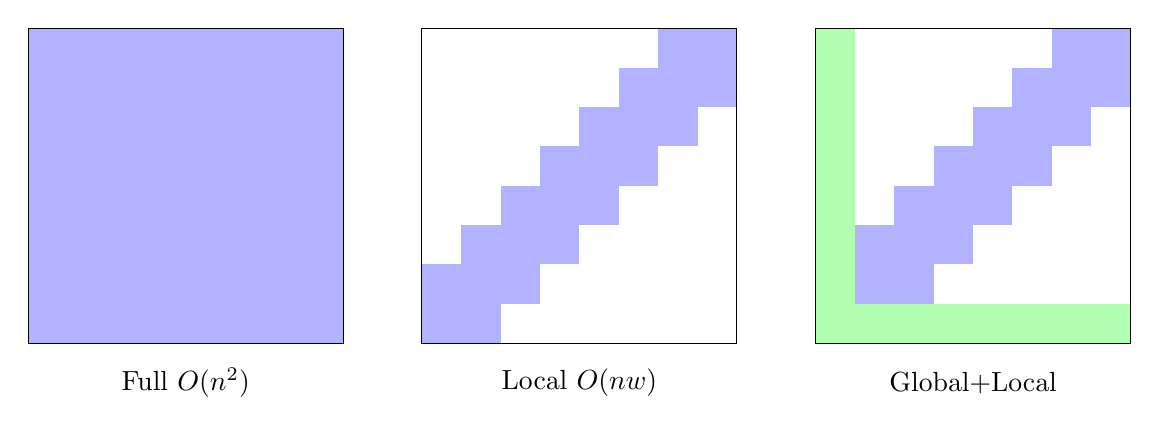
\begin{tikzpicture}[scale=0.5]
    % Full attention
    \begin{scope}[shift={(0,0)}]
        \fill[blue!30] (0,0) rectangle (8,8);
        \draw (0,0) rectangle (8,8);
        \node at (4, -1) {Full $O(n^2)$};
    \end{scope}

    % Local attention
    \begin{scope}[shift={(10,0)}]
        \foreach \i in {0,...,7} {
            \fill[blue!30] ({max(0,\i-1)}, \i) rectangle ({min(8,\i+2)}, {\i+1});
        }
        \draw (0,0) rectangle (8,8);
        \node at (4, -1) {Local $O(nw)$};
    \end{scope}

    % Global + Local
    \begin{scope}[shift={(20,0)}]
        \foreach \i in {0,...,7} {
            \fill[blue!30] ({max(0,\i-1)}, \i) rectangle ({min(8,\i+2)}, {\i+1});
        }
        \fill[green!30] (0,0) rectangle (8,1);
        \fill[green!30] (0,0) rectangle (1,8);
        \draw (0,0) rectangle (8,8);
        \node at (4, -1) {Global+Local};
    \end{scope}
\end{tikzpicture}
\caption{Different attention patterns. Blue = local attention, Green = global attention.}
\label{fig:attention_patterns}
\end{figure}

\subsection{Linear Attention}

\textbf{Key idea.} Replace the softmax with a decomposable kernel $\phi(\vq)^T \phi(\vk)$, enabling the computation to be rearranged from $O(n^2 d)$ to $O(n d^2)$---linear in sequence length.

\textbf{Trade-off.} Approximation quality varies; often lower quality than full attention. Examples: Performer, Linear Transformer.

\textbf{In practice.} Flash Attention has largely made linear attention unnecessary for moderate sequence lengths ($<$ 32K). Linear attention is mainly relevant for very long sequences where even Flash Attention's $O(n^2)$ compute is prohibitive.

\subsection{Multi-Query Attention (MQA)}

\begin{mathresult}{Multi-Query Attention}
Share keys and values across all attention heads:
\begin{align}
\mQ_i &= \mX \mW_i^Q \quad \text{(per head)} \\
\mK &= \mX \mW^K \quad \text{(shared)} \\
\mV &= \mX \mW^V \quad \text{(shared)}
\end{align}
\end{mathresult}

\textbf{Benefit}: KV cache reduced by factor of $h$ (number of heads).

\textbf{Used in}: PaLM, Falcon

\subsection{Grouped-Query Attention (GQA)}

\begin{mathresult}{Grouped-Query Attention}
Middle ground: Share K/V within groups of heads.
\begin{itemize}
    \item $h$ query heads
    \item $g$ key-value heads (where $g$ divides $h$)
    \item Each K/V head shared by $h/g$ query heads
\end{itemize}
\end{mathresult}

\textbf{Example}: 32 query heads, 8 KV heads = 4$\times$ KV cache reduction

\textbf{Used in}: LLaMA 2, Mistral

\begin{table}[H]
\centering
\caption{Attention variant comparison}
\begin{tabularx}{\textwidth}{lXXX}
\toprule
\textbf{Variant} & \textbf{KV Heads} & \textbf{Quality} & \textbf{Inference Speed} \\
\midrule
Multi-Head (MHA) & $h$ & Best & Baseline \\
Grouped-Query (GQA) & $g < h$ & Very good & Faster \\
Multi-Query (MQA) & 1 & Good & Fastest \\
\bottomrule
\end{tabularx}
\end{table}

\subsection{Flash Attention}

\begin{keyinsight}{Why Flash Attention Matters}
Flash Attention is not a different attention mechanism---it computes \textbf{exactly the same result} as standard attention, but with better memory efficiency through careful tiling.
\end{keyinsight}

\subsubsection{The Memory Bottleneck}

Standard attention materializes the full $n \times n$ attention matrix in GPU HBM (high bandwidth memory). But GPU SRAM (fast on-chip memory) is much smaller (20 MB vs 40 GB on A100). The bottleneck is memory I/O, not compute.

\subsubsection{Flash Attention Approach}

\begin{enumerate}
    \item Process in tiles that fit in SRAM (fast memory)
    \item Compute softmax incrementally (online softmax)
    \item Never materialize full $n \times n$ attention matrix
\end{enumerate}

\textbf{Online Softmax Trick}:
\begin{equation}
\softmax([x_1, \ldots, x_n])_i = \frac{e^{x_i - m}}{e^{x_1 - m} + \cdots + e^{x_n - m}}
\end{equation}
where $m = \max_j x_j$. Can be computed incrementally as blocks arrive.

\subsubsection{Benefits}

\begin{itemize}
    \item \textbf{Memory}: $O(n)$ instead of $O(n^2)$
    \item \textbf{Speed}: 2-4$\times$ faster (memory-bound $\to$ compute-bound)
    \item \textbf{Exact}: Same numerical result as standard attention
\end{itemize}

\textbf{Used in}: Essentially all modern LLM training and inference

\begin{interviewq}
\textbf{Q: Explain Flash Attention. Why is it faster even though it does the same computation?}

\textbf{What the interviewer is testing:} Understanding of hardware-aware algorithm design, memory hierarchy (SRAM vs HBM), and the difference between compute-bound and memory-bound operations.

\textbf{A:} Flash Attention computes \textit{exactly} the same result as standard attention, but reorganizes the computation to minimize memory I/O:

\begin{enumerate}
    \item \textbf{Problem}: Standard attention materializes the full $n \times n$ matrix in slow HBM memory. The bottleneck is reading/writing this matrix, not computing it.
    \item \textbf{Solution}: Process attention in tiles that fit in fast SRAM. Use the online softmax trick to compute exact softmax incrementally without ever materializing the full matrix.
    \item \textbf{Result}: Memory drops from $O(n^2)$ to $O(n)$. Speed improves 2-4$\times$ because operations become compute-bound rather than memory-bound.
\end{enumerate}

\textbf{Common follow-ups:} ``What's the online softmax trick?'' ``When would Flash Attention NOT help?'' (Small sequences where attention isn't the bottleneck.)
\end{interviewq}

%==============================================================================
\section{Modern Transformer Design Choices}
\label{sec:modern_design}
%==============================================================================

\subsection{Architecture Comparison: GPT-2 vs LLaMA}

\begin{table}[H]
\centering
\caption{Evolution of Transformer design choices}
\begin{tabularx}{\textwidth}{lXX}
\toprule
\textbf{Component} & \textbf{GPT-2 (2019)} & \textbf{LLaMA (2023)} \\
\midrule
Normalization & LayerNorm & RMSNorm \\
Norm placement & Post-norm & Pre-norm \\
Position encoding & Learned & RoPE \\
Activation & GELU & SwiGLU \\
Attention & Multi-head & Grouped-query (LLaMA 2) \\
Bias terms & Yes & No \\
\bottomrule
\end{tabularx}
\end{table}

\subsection{RMSNorm vs LayerNorm}

\textbf{LayerNorm}:
\begin{equation}
\text{LN}(\vx) = \frac{\vx - \mu}{\sigma} \odot \bm{\gamma} + \bm{\beta}
\end{equation}

\textbf{RMSNorm}:
\begin{equation}
\text{RMS}(\vx) = \frac{\vx}{\sqrt{\frac{1}{d}\sum_i x_i^2}} \odot \bm{\gamma}
\end{equation}

\textbf{Benefits of RMSNorm}:
\begin{itemize}
    \item No mean computation (simpler)
    \item Empirically similar performance
    \item ~10-15\% faster
\end{itemize}

\subsection{SwiGLU Activation}

\begin{mathresult}{SwiGLU Feed-Forward Network}
\begin{equation}
\text{FFN}_{SwiGLU}(\vx) = (\text{Swish}(\vx\mW_1) \odot \vx\mV) \mW_2
\end{equation}
where $\text{Swish}(x) = x \cdot \sigma(x)$ and $\odot$ is element-wise multiplication.
\end{mathresult}

\textbf{Compared to standard FFN}:
\begin{equation}
\text{FFN}_{standard}(\vx) = \text{GELU}(\vx\mW_1)\mW_2
\end{equation}

\textbf{SwiGLU benefits}:
\begin{itemize}
    \item Gating provides multiplicative interaction
    \item Better empirical performance
    \item Note: Uses 3 weight matrices instead of 2, so expansion factor adjusted (8/3 instead of 4)
\end{itemize}

\subsection{KV Cache for Inference}

For autoregressive generation, recomputing attention for all previous tokens is wasteful.

\textbf{KV Cache}: Store keys and values from previous positions.

For position $t$:
\begin{align}
\vk_t &= \vx_t \mW^K \quad \to \quad \text{append to } \mK_{cache} \\
\vv_t &= \vx_t \mW^V \quad \to \quad \text{append to } \mV_{cache} \\
\vq_t &= \vx_t \mW^Q \\
\text{attn}_t &= \softmax\left(\frac{\vq_t \mK_{cache}^T}{\sqrt{d_k}}\right) \mV_{cache}
\end{align}

\textbf{Memory requirement} (per sequence):
\begin{equation}
2 \times L \times n_{layers} \times n_{heads} \times d_{head} \times \text{bytes per element}
\end{equation}

\begin{example}[LLaMA 7B KV Cache]
\begin{itemize}
    \item 32 layers, 32 heads, 128 dim per head
    \item 2K context, FP16
    \item $2 \times 2048 \times 32 \times 32 \times 128 \times 2$ bytes $\approx$ 1 GB per sequence
\end{itemize}
\end{example}

\begin{warningbox}
KV cache memory grows linearly with sequence length and batch size. For LLaMA 7B with 2K context in FP16, each sequence needs $\sim$1 GB of KV cache. At 32K context, that's $\sim$16 GB per sequence---easily exceeding GPU memory. This is why KV cache compression (quantization, eviction, PagedAttention) is critical for long-context inference.
\end{warningbox}

%==============================================================================
\section{Computational Analysis}
\label{sec:transformer_compute}
%==============================================================================

\subsection{Parameter Count}

For a Transformer with:
\begin{itemize}
    \item $L$ layers
    \item $d$ model dimension
    \item $h$ attention heads
    \item FFN expansion factor $f$ (typically 4)
    \item Vocabulary size $V$
\end{itemize}

\begin{align}
\text{Embedding} &: V \times d \\
\text{Per layer attention} &: 4d^2 \quad (\mW^Q, \mW^K, \mW^V, \mW^O) \\
\text{Per layer FFN} &: 2 \times d \times fd = 2fd^2 \quad (\mW_1, \mW_2) \\
\text{Per layer norm} &: 2 \times 2d = 4d \quad (\text{2 LayerNorms}) \\
\text{Total per layer} &\approx 4d^2 + 2fd^2 = (4 + 2f)d^2 \\
\text{Total} &\approx L(4 + 2f)d^2 + Vd
\end{align}

With $f=4$: Parameters $\approx 12Ld^2 + Vd$

\subsection{FLOPs per Token}

For a forward pass with sequence length $n$:

\begin{align}
\text{Attention Q,K,V projection} &: 3 \times 2nd^2 = 6nd^2 \\
\text{Attention scores} &: 2n^2d \\
\text{Attention output} &: 2n^2d + 2nd^2 \\
\text{FFN} &: 2 \times 2 \times nd \times fd = 4fnd^2 \\
\text{Per layer total} &\approx (8 + 4f)nd^2 + 4n^2d
\end{align}

With $f=4$: FLOPs per layer $\approx 24nd^2 + 4n^2d$

\textbf{Observation}: For large $n$, the $n^2$ term dominates (attention). For typical LLM inference (small $n$), the $nd^2$ term dominates (projections).

\begin{interviewq}
\textbf{Q: Estimate the memory required to train a 7B parameter model with batch size 1, sequence length 2048.}

\textbf{What the interviewer is testing:} Can you do back-of-envelope calculations for ML systems? Do you know the memory components of training (parameters, gradients, optimizer states, activations)?

\textbf{A:} Memory components:
\begin{enumerate}
    \item \textbf{Parameters}: 7B $\times$ 4 bytes (FP32) = 28 GB
    \item \textbf{Gradients}: 7B $\times$ 4 bytes = 28 GB
    \item \textbf{Optimizer states (Adam)}: 7B $\times$ 8 bytes = 56 GB (momentum + variance)
    \item \textbf{Activations}: Roughly 2--4$\times$ parameter count for typical models $\approx$ 56--112 GB
\end{enumerate}

Total: ~168-224 GB minimum

\textbf{Solutions for limited memory}:
\begin{itemize}
    \item Mixed precision (FP16/BF16): Halves parameter/gradient memory
    \item Gradient checkpointing: Trade compute for activation memory
    \item ZeRO: Distribute optimizer states across GPUs
    \item Gradient accumulation: Smaller effective batch size per step
\end{itemize}
\end{interviewq}

\begin{interviewq}
\textbf{Q: How does RoPE encode position information? Why is it preferred over learned positional embeddings?}

\textbf{What the interviewer is testing:} Whether you understand how modern LLMs handle position, and the extrapolation problem.

\textbf{A:} RoPE rotates query and key vectors by an angle proportional to their position. The dot product of rotated Q and K naturally depends only on their relative position (because $R_m^T R_n = R_{n-m}$).

Three advantages over learned embeddings:
\begin{itemize}
    \item \textbf{Relative position for free}: No separate relative position mechanism needed.
    \item \textbf{Extrapolation}: Can extend to longer sequences than training (with techniques like NTK-aware scaling or YaRN).
    \item \textbf{No extra parameters}: Position information is injected through rotation, not additional embeddings.
\end{itemize}

\textbf{Common follow-ups:} ``How would you extend a RoPE-based model trained on 4K context to 32K?'' (NTK-aware interpolation, YaRN, or progressive training on longer contexts.)
\end{interviewq}

\begin{interviewq}
\textbf{Q: What is Grouped-Query Attention and why does LLaMA 2 use it?}

\textbf{What the interviewer is testing:} Understanding of inference optimization, KV cache memory, and quality-speed trade-offs.

\textbf{A:} GQA shares key-value heads among groups of query heads. LLaMA 2 uses 32 query heads but only 8 KV heads, meaning each KV head is shared by 4 query heads.

\textbf{Why it matters for inference:}
\begin{itemize}
    \item KV cache stores past keys and values for autoregressive generation.
    \item With standard MHA, KV cache = $2 \times n_{layers} \times n_{heads} \times d_{head} \times \text{seq\_len} \times \text{bytes}$.
    \item GQA with 8 instead of 32 KV heads gives a $4\times$ reduction in KV cache memory.
    \item This means you can serve more concurrent users or longer sequences with the same GPU memory.
\end{itemize}

Quality loss is minimal---GQA performs nearly as well as full MHA, much better than MQA (1 KV head).

\textbf{Common follow-ups:} ``How would you convert an MHA model to GQA?'' (Average the KV heads within each group during conversion, then fine-tune.)
\end{interviewq}
